\documentclass[a4paper,12pt]{article}

\usepackage[left=1in, right=1in, top=0.5in, bottom=1in]{geometry}
\usepackage[latin2]{inputenc} \usepackage{amsmath}
\usepackage{graphicx} \usepackage[T1]{fontenc} \usepackage{color}
\usepackage{amssymb} \usepackage{times}

\newcommand{\lhood}{\ensuremath{\mathcal{L}}}
\newcommand{\truth}{\ensuremath{\mathcal{T}}}
\newcommand{\model}{\ensuremath{\mathcal{M}}}
\newcommand{\optmodel}{\ensuremath{\mathcal{M}^*}}

\DeclareMathOperator*{\argmin}{arg\,min}
\DeclareMathOperator*{\argmax}{arg\,max}

% Some useful macros

\definecolor{Cgreen}{rgb}{0,0.6,0}
\definecolor{Cblue}{rgb}{0,0.39,0.61}

\newcounter{ohNoteCounter} \newcommand{\ohnote}[1]{{\scriptsize
    \color{Cgreen}
    $\clubsuit$~\refstepcounter{ohNoteCounter}\textsf{[OH]$_{\arabic{ohNoteCounter}}$:{#1}}}}

\newcounter{jpNoteCounter} \newcommand{\jpnote}[1]{{\scriptsize
    \color{Cblue} $\blacksquare$
    \refstepcounter{jpNoteCounter}\textsf{[JP]$_{\arabic{jpNoteCounter}}$:{#1}}}}

\IfFileExists{.notes_disabled}{ \renewcommand{\jpnote}[1]{}
  \renewcommand{\ohnote}[1]{} }

\title { \normalsize Graphical Markov Models \\ Winter 2011 \\
 \vspace{10mm} {\bf Identifying License Plates with Hidden Markov
    Models } }
\author{\normalsize James Pritts and Ondra Hrstka }
\date{ \small November 2011 }

\begin{document}
\maketitle

\pagestyle{empty} \ohnote{This is useful way to leave notes. Both of
  us have command tu leave notes. I have \textbackslash ohnote, you
  have \textbackslash jpnote. Notes in whole document can be disabled
  by creating file with name ``.notes\_disabled''. }

\section{Problem Statement}
The problem is to report the unique identifying string of characters,
called the \emph{vehicle-id}, of a license plate.  Provided are images
of license plates that have been segmented and ortho-rectified. A
subset of these images each have the following corresponding
annotations: a top and bottom boundary that delimits the vehicle-id
within the segmented license plate, a bounding box of each character
and white-space interval that comprises the vehicle-id, and a
character label for each bounding box that contains a character.  We
assume that the font of all characters across license plates is
identical, and we refer to a particular character of the font set as a
glyph.

\section{Preliminaries}
Let $I\colon \mathbb{Z}^2_+ \to \mathbb{R}$ be a function that maps a
point $\mathbf{u} = (i,j)$ to a real value $x_{ij}$, such that $I$
gives the raw intensity value at each point in the image.  Denote
$\mathbf{x}_i$ and $\mathbf{x}_j$ as the row and column of pixels in
the image at row $i$ and column $j$ respectively.

To condense the notation for probability distributions, we denote
$p_{x_{ij} \mid s_j}(x_{ij} \mid s_j)$ by writing $p(x_{ij} \mid
s_j)$; in other words, the arguments of $p$ will uniquely select the
proper density function for evaluation.

\section{Model Definition}
We model a \emph{vehicle-id} by a Hidden Markov Model (\textbf{HMM}).
The characters of the \emph{vehicle-id} are assumed to come from the
same font set, so any image of a particular character can be mapped to
the same glyph.  The left-to-right sequence of consecutive columns
from the segmented license plate are the \emph{observations}.

The set of \emph{hidden states} $\mathbf{K}$ are the column indices of
all the glyphs in the font set and an added state $w$ that represents
white-space. An example sequence of hidden states $S \in \mathbf{K}^n$
is
\[S =
\left(\,\dots,\text{w},\text{A}_1,\text{A}_2,\ldots,\text{A}_{m},\text{w},\text{w},\text{w},\text{T}_1,\text{T}_2,\ldots\,\right).\]

The \emph{emission probabilities} are the probabilities of observing
pixel intensities given their corresponding glyph column, or,
equivalently, given their \emph{hidden states}. We make the
simplifying assumption that probabilities of observing intensities in
a column $\mathbf{x}_j$ are pairwise independent \[p(\mathbf{x}_j \mid
s_j) = \prod_{i=1}^np(x_{ij} \mid s_j).\] The probability of observing
pixel intensity $x_{ij}$ of a glyph column $s_j$ is modeled as a
two-class gaussian mixture, where the first class $c=f$ contains
foreground pixels, and the second class $c=b$ contains background
pixels,
\begin{align*}
  p(x_{ij} \mid s_j) &= p(x_{ij},c=f \mid s_j)+p(x_{ij},c=b \mid s_j)\\
  &= p(x_{ij}\mid c=f,s_j)p(c=f \mid s_j)+p(x_{ij} \mid c=b,s_j)p(c=b \mid s_j) \\
  &= p(x_{ij}\mid c=f)p(c=f \mid s_j)+p(x_{ij} \mid c=b)p(c=b \mid s_j) \\
  &= \mathcal{N}(\sigma_1,\mu_1)\gamma_{is_j}+\mathcal{N}(\sigma_2,\mu_2)(1-\gamma_{is_j}).
\end{align*}
The model for \emph{emissions probabilities} assumes that the
foreground and background distributions are position independent,
while the mixture parameter depends on the row position of the glyph
column $s_j$.

\section{Learning}
The annotated data $\truth$ does not contain segmentations of
vehicle-id characters from the background.  \emph{Unsupervised
  learning} will be required to specify the \emph{emissions
  probabilities}.  

Denote the set of parameters needed to determine the model of a glyph
column as
\[\model_{k_j}=\{\,\mu_1,\sigma_1,\mu_2,\sigma_2,\gamma_{1,k_j},\gamma_{2,k_j},\ldots,\gamma_{m,k_j}\,\}.\]
Then the model for all columns of all glyphs in the entire font set is
specified as
\[
\model = \cup_{i=1}^m\model_{k_i}.
\]
Given the annotated data $\truth$, we seek the maximum-likelihood
estimate \[ \optmodel = \argmax_{\model} \lhood(\truth \mid \model)\].



for each glyph column $k_j \in \mathbf{K}$ from the annotated image
data, Learning a model for a glyph column comprises of learning the
position-independent global foreground $ p(x_{ij}\mid
c=f,s_j)=\mathcal{N}(\sigma_1,\mu_1)$ and background $p(x_{ij} \mid
c=b,s_j)=\mathcal{N}(\sigma_2,\mu_2)$ image intensity models, as well
their position-dependent and glyph-dependent priors.

% \begin{algorithm}
%   \Input{A set of images $I_n$} \Output{Maximum likelihood estimate
%   of parameters $\gamma_{i \in 1:n},\mu_f,\sigma_f,\mu_b\sigma_b$}
%
%
%
% \end{algorithm}
%

See something on figure \ref{fig:some-label}
\begin{figure}[htp]
\centering
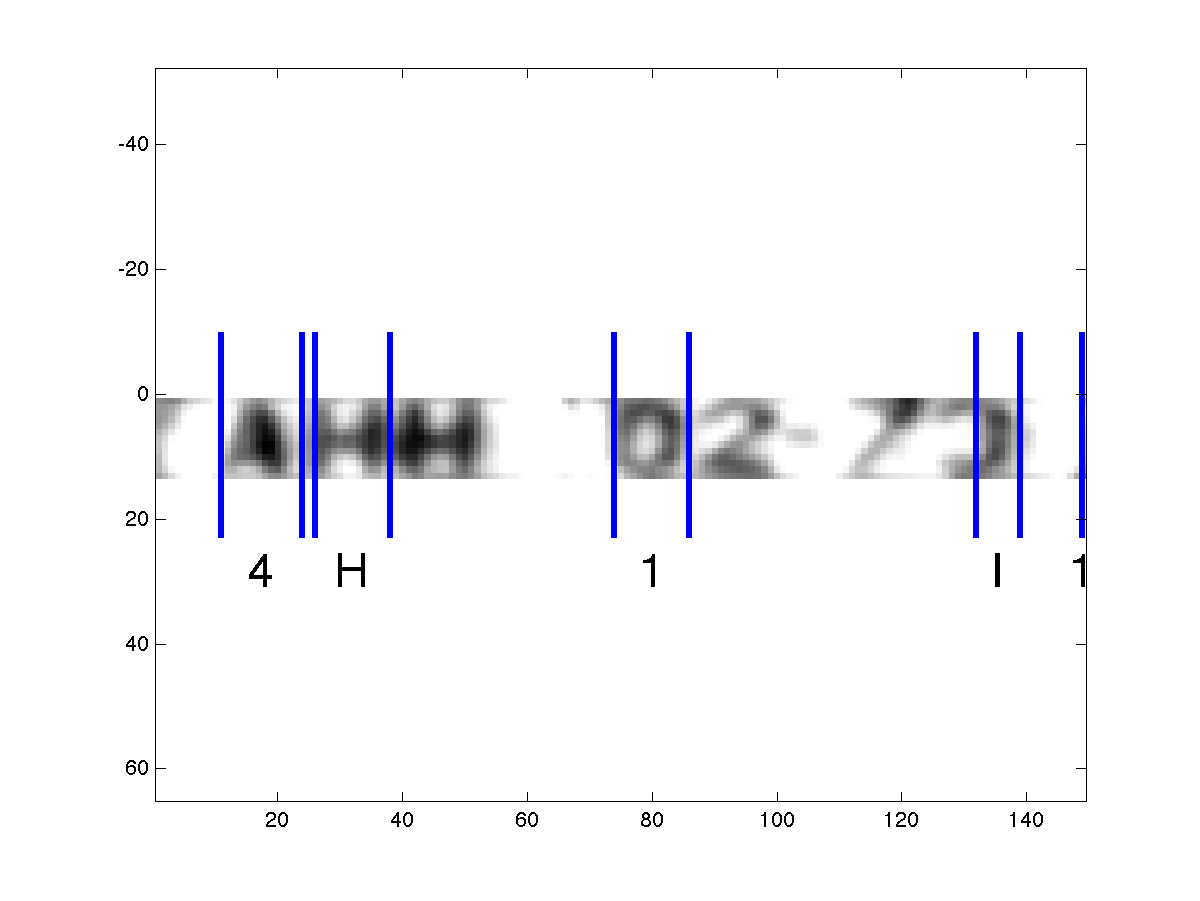
\includegraphics[width=\linewidth]{pics/detection.png}
\caption{Bla bla bla bla bla} 
\label{fig:some-label}
\end{figure}

\end{document}

